\section{Programmiersprachen}
\setauthor{Felix Dumfarth}

\subsection{Java}
\setauthor{Felix Dumfarth}

\begin{figure}[hbt!]
    \centering
    
\includegraphics[scale=0.5]{pics/java}
    \caption{Java Logo\cite{java}}
    \label{fig:impl:java}
\end{figure}

Für das Backend wurde sich für Java entschieden.
Java ist nach dem TIOBE-Index ~\cite{tiobe} eine der populärsten Programmiersprachen.
Java ist eine für Menschen sehr einfach lesbare Sprache, aber damit Maschinen sie auch lesen können, wird ein Java-Compiler, der den Code in Java-Bytecode umwandelt, benötigt.
Ohne diesen Vorgang kann der Code nicht ausgeführt werden.
Java ist eine sogenannte objektorientierte Programmiersprache und besitzt dadurch Klassen und Vererbung\cite{java}.

\subsection{Python}
\setauthor{Felix Dumfarth}

Python ist eine Programmiersprache, die mehrere Arten der Programmierung wie die objektorientierte, die aspektorientierte und die funktionale Programmierung unterstützt.
Es handelt sich hier um eine Programmiersprache, die versucht, einen knappen und dadurch gut lesbaren Programmierstil zu besitzen.
Python wird oft für Machine Learning verwendet.
Auch bei dieser Arbeit wurde Python zusammen mit Rasa verwendet.
Zum einen ist Rasa ein Python-Framework und zum anderen werden die Custom Actions mit Python umgesetzt.

\subsection{TypeScript}
TypeScript wurde im Jahr 2012 von Microsoft entwickelt und ist eine Programmiersprache, die eine kompakte und einfache Syntax zur Programmierung von Webseiten und Anwendungen bietet.
Typescript baut auf JavaScript auf und hilft zum Beispiel beim frühzeitigen Erkennen von Fehlern.
Bei TypeScript wird mit Unterstützung von Modulen das Kapseln von Klassen, Interfaces, Funktionen und Variablen in eigene Namensräume ermöglicht.
Es gibt hierbei eine Unterscheidung zwischen internen und externen Modulen.

\section{Technologien}
\setauthor{Felix Dumfarth}

\subsection{REST Service}
\setauthor{Felix Dumfarth}

REST ist die Abkürzung für Representational State Transfer.
REST Anfragen sind sogenannte CRUD–Operationen.
Darunter fallen die Operationen \texttt{Create}, \texttt{Read}, \texttt{Update} und \texttt{Delete}.
Diese sind GET, POST, PUT und DELETE Requests.
Außerdem gibt es noch OPTIONS, PATCH, HEAD, TRACE und CONNECT\@.
Diese werden aber in der vorliegenden Arbeit nicht benutzt.

\begin{itemize}
    \item Die GET Methode ist zuständig für das Abfragen von Daten.
    Dabei soll ein Request geschickt werden und es werden nur Daten zurückgeben.
    Auf dem Server, zu dem die Anfrage geschickt wird, soll nichts geschehen außer das Lesen von Daten und das anschließende Zurückgeben dieser.
    \item Bei POST sollen Daten hinzugefügt werden.
    Im Normalfall ist in der Response der URI der neu gespeicherten Daten.
    \item Bei PUT werden Daten hinzugefügt.
    Falls diese schon existieren, werden sie upgedatet und falls nicht, wird ein neuer Eintrag erstellt.
    \item Bei DELETE werden Daten gelöscht.
\end{itemize}

\subsection{Quarkus}\label{quarkus}
\setauthor{Felix Dumfarth}

Quarkus ist ein Java-Framework, welches auf die REST-Service-API ausgerichtet ist.
Das Backend ~\ref{sec:backend} wurde mit Quarkus umgesetzt.

\subsection{Angular}
\setauthor{Felix Dumfarth}

Angular basiert auf TypeScript und ist ein Framework für Webseiten.
Dieses ist ausgelegt für Single Page Applications.
Das Chat Widget ~\ref{sec:chat-widget} und das Dashboard ~\ref{sec:dashboard} wurden mit Angular umgesetzt

\subsection{Angular Elements}\label{subsec:angular-elements}
\setauthor{Felix Dumfarth}

''Webkomponenten sind eine Gruppe von Web-Technologien, die es ermöglichen, benutzerdefinierte, wiederverwendbare HTML Elemente zu erstellen, deren Funktionalität gekapselt ist und damit vollständig getrennt von anderem Code.''\cite{webcomponents}

Um die Chatkomponente auf die WordPress Seite zu bringen, wurde entschieden, dass die Komponente mithilfe von Angular Elements als Webkomponente exportiert wird, um somit eine einfache Einbindung auf die Schulhomepage zu ermöglichen.

Eine Webkomponente wird in Angular Elements in 3 Javascript Files erstellt.
Diese sind:

\begin{enumerate}
    \item main.js
    \item polyfills.js
    \item runtime.js
\end{enumerate}

Dabei können diese drei Komponenten jedoch ohne Bedenken zu einem einzelnen JavaScript File zusammengefasst werden.

Um die Webkomponente in HTML zu benutzen, müssen alle JS-Dateien eingebunden werden und schon kann die eigene Komponente wie jedes andere Element benutzt werden.

\begin{lstlisting}[language=html,label={lst:webcomponent},caption={HTML File}]{HTML File}]
...
<name-der-komponente></name-der-komponente>

<script src="./runtime.js"></script>
<script src="./polyfills.js"></script>
<script src="./main.js"></script>
...
\end{lstlisting}

\section{Werkzeuge}
\setauthor{Felix Dumfarth}

\subsection{Rasa X}\label{subsec:rasa-x}
Rasa X ist ein Werkzeug, um Conversation-Driven Development ~\ref{cdd} in die Tat umzusetzen.\cite{rasax}
Rasa X liefert erweiterte Funktionalitäten zu einem Rasa-Chatbot, die nur mit Rasa alleine nicht gegeben sind.
Rasa X wurde mit Docker Compose ~\cite{rasaxDocker} auf der VM installiert ~\ref{sec:systemarchitektur}.

Rasa X bietet dazu eine grafische Weboberfläche an.
Auf dieser können Intents ~\ref{subsec:Intents}, Responses ~\ref{subsec:Responses}, etc. angesehen und verändert werden.
Außerdem besteht die Möglichkeit, ein eigenes Model zu trainieren oder ein Model hochzuladen.

Da jedoch ein eigenes Dashboard im Rahmen dieser Diplomarbeit verwendet wird, wird die grafische Oberfläche nicht benötigt, sondern nur die erweiterte Funktionalität, die auch über die API aufgerufen werden kann.

Damit das Frontend auf Rasa, welches eine Ebene unter Rasa X liegt, zugreifen kann, muss das automatisch erstellte \texttt{credentials.yml} File bearbeitet werden.
Dies ist in Listing ~\ref{lst:rasaXCred} beschrieben.

\begin{lstlisting}[language=yaml,label={lst:rasaXCred},caption={credentials.yml}]{credentials.yml}]
rasa:
url: ${RASA_X_HOST}/api
rest:
\end{lstlisting}

Eine Herausforderung stellte dabei das Verschlüsseln der Kommunikation mit Rasa X mithilfe von HTTPS dar.
Es wird ein Zertifikat benötigt.
Hierbei ist es möglich, ein Zertifikat mithilfe des Certbots ~\cite{certbot} zu erstellen.
Diese Zertifikate müssen dann in den \texttt{certs} Ordner gegeben werden.

\begin{lstlisting}[language=bash,label={lst:certbot},caption={Install certbot and create certificates}]{certbot}]
sudo ln -s /snap/bin/certbot /usr/bin/certbot
sudo certbot certonly -d vm45.htl-leonding.ac.at
sudo cp /etc/letsencrypt/live/vm45.htl-leonding.ac.at/privkey.pem /etc/rasa/certs/
sudo cp /etc/letsencrypt/live/vm45.htl-leonding.ac.at/fullchain.pem /etc/rasa/certs/
sudo chmod 640 certs/privkey.pem
\end{lstlisting}

Außerdem müssen beim Nginx Server noch diverse Einstellungen vorgenommen werden.
In dem File \texttt{nginx-config-files/rasax.nginx.template} muss die Zeile mit ``include'' auskommentiert werden.

\begin{lstlisting}[language=yaml,label={lst:rasaxnginxtemplate},caption={rasax.nginx.template}]{rasax.nginx.template}]
...
server {
    listen            8080;
    include           /etc/nginx/conf.d/ssl.conf;
    ...
\end{lstlisting}

Und in \texttt{nginx-config-files/ssl.conf.template} müssen die Zeilen, wie in Listing ~\ref{lst:sslconftemplate} beschrieben, auskommentiert werden.

\begin{lstlisting}[language=yaml,label={lst:sslconftemplate},caption={ssl.conf.template}]{ssl.conf.templatte}]
listen                  8443 ssl;

# server_name           example.com;
ssl_certificate         /etc/certs/fullchain.pem;
ssl_certificate_key     /etc/certs/privkey.pem;
\end{lstlisting}

Nun muss Rasa X gestoppt und wieder hochgefahren werden, um die neuen Einstellungen zu übernehmen.

\subsection{IntelliJ IDEA}
IntelliJ ist ein IDE, welches eine Vielzahl von Programmiersprachen unterstützt und hauptsächlich für diese Arbeit verwendet wird.

\subsection{GitHub}
GitHub ist ein Online-Repository, welches die gemeinsame Programmierung von Anwendungen erleichtert.

\subsection{GitHub Actions}\label{subsec:github-actions}
Mit GitHub Actions können Workflows für ein GitHub Repository erstellt werden.
Ein Workflow besteht aus einem oder mehreren Jobs, wobei ein Job aus einem oder mehreren Schritten besteht.

\begin{figure}[hbt!]
    \centering
    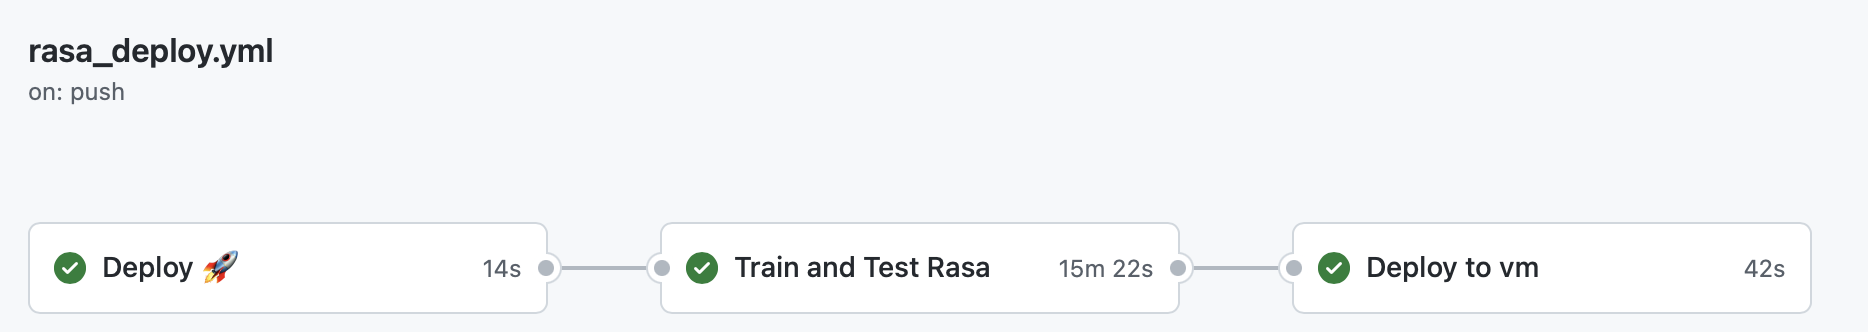
\includegraphics[scale=0.5]{pics/ghActions}
    \caption{Beispiel eines Workflows}
    \label{fig:impl:ghActions}
\end{figure}

Die Jobs werden dabei automatisch abgearbeitet und meistens wird am Ende des Workflows das Produkt auf einen Server geladen.
Bei jeder Action wird standardmäßig ein checkout benutzt:

\begin{lstlisting}[language=yaml,label={lst:checkout},caption={In der Action}]{In der Action}]
...
jobs:
  build:
    runs-on: ubuntu-latest
    steps:
      - name: Checkout
        uses: actions/checkout@v2
...
\end{lstlisting}

Checkout sorgt dabei dafür, dass der Workflow auf das Projekt zugreifen kann.

\subsection{Docker}
Docker ist ein Container-Manager, der es erlaubt Anwendungen zu isolieren.
Dies wird in sogenannten Docker-Containern gemacht.

\subsection{WordPress}
WordPress ist ein freies und open-source Content-Management-System, das in PHP geschrieben ist.
Für die Speicherung der Daten wird entweder eine MySQL oder eine MariaDB Datenbank verwendet.
WordPress verwendet Plugins für die Erweiterung der Funktionalitäten und Themes für die Anpassung des Designs.
Das CMS wurde ursprünglich für das Erstellen von Blogs benutzt, hat sich jedoch inzwischen zu einem System für das Verwalten verschiedenster Web-Inhalte entwickelt.
Mit einem Marktanteil von 42,8\% der 10 Millionen meistbesuchten Websites ist WordPress das beliebteste Content-Management-System.

Die HTL Leonding Schulhomepage wurde mithilfe von WordPress gemacht, deshalb war es wichtig, dass das Endprodukt der Arbeit auch mit WordPress kompatibel ist.


\begin{figure}[hbt!]
    \centering
    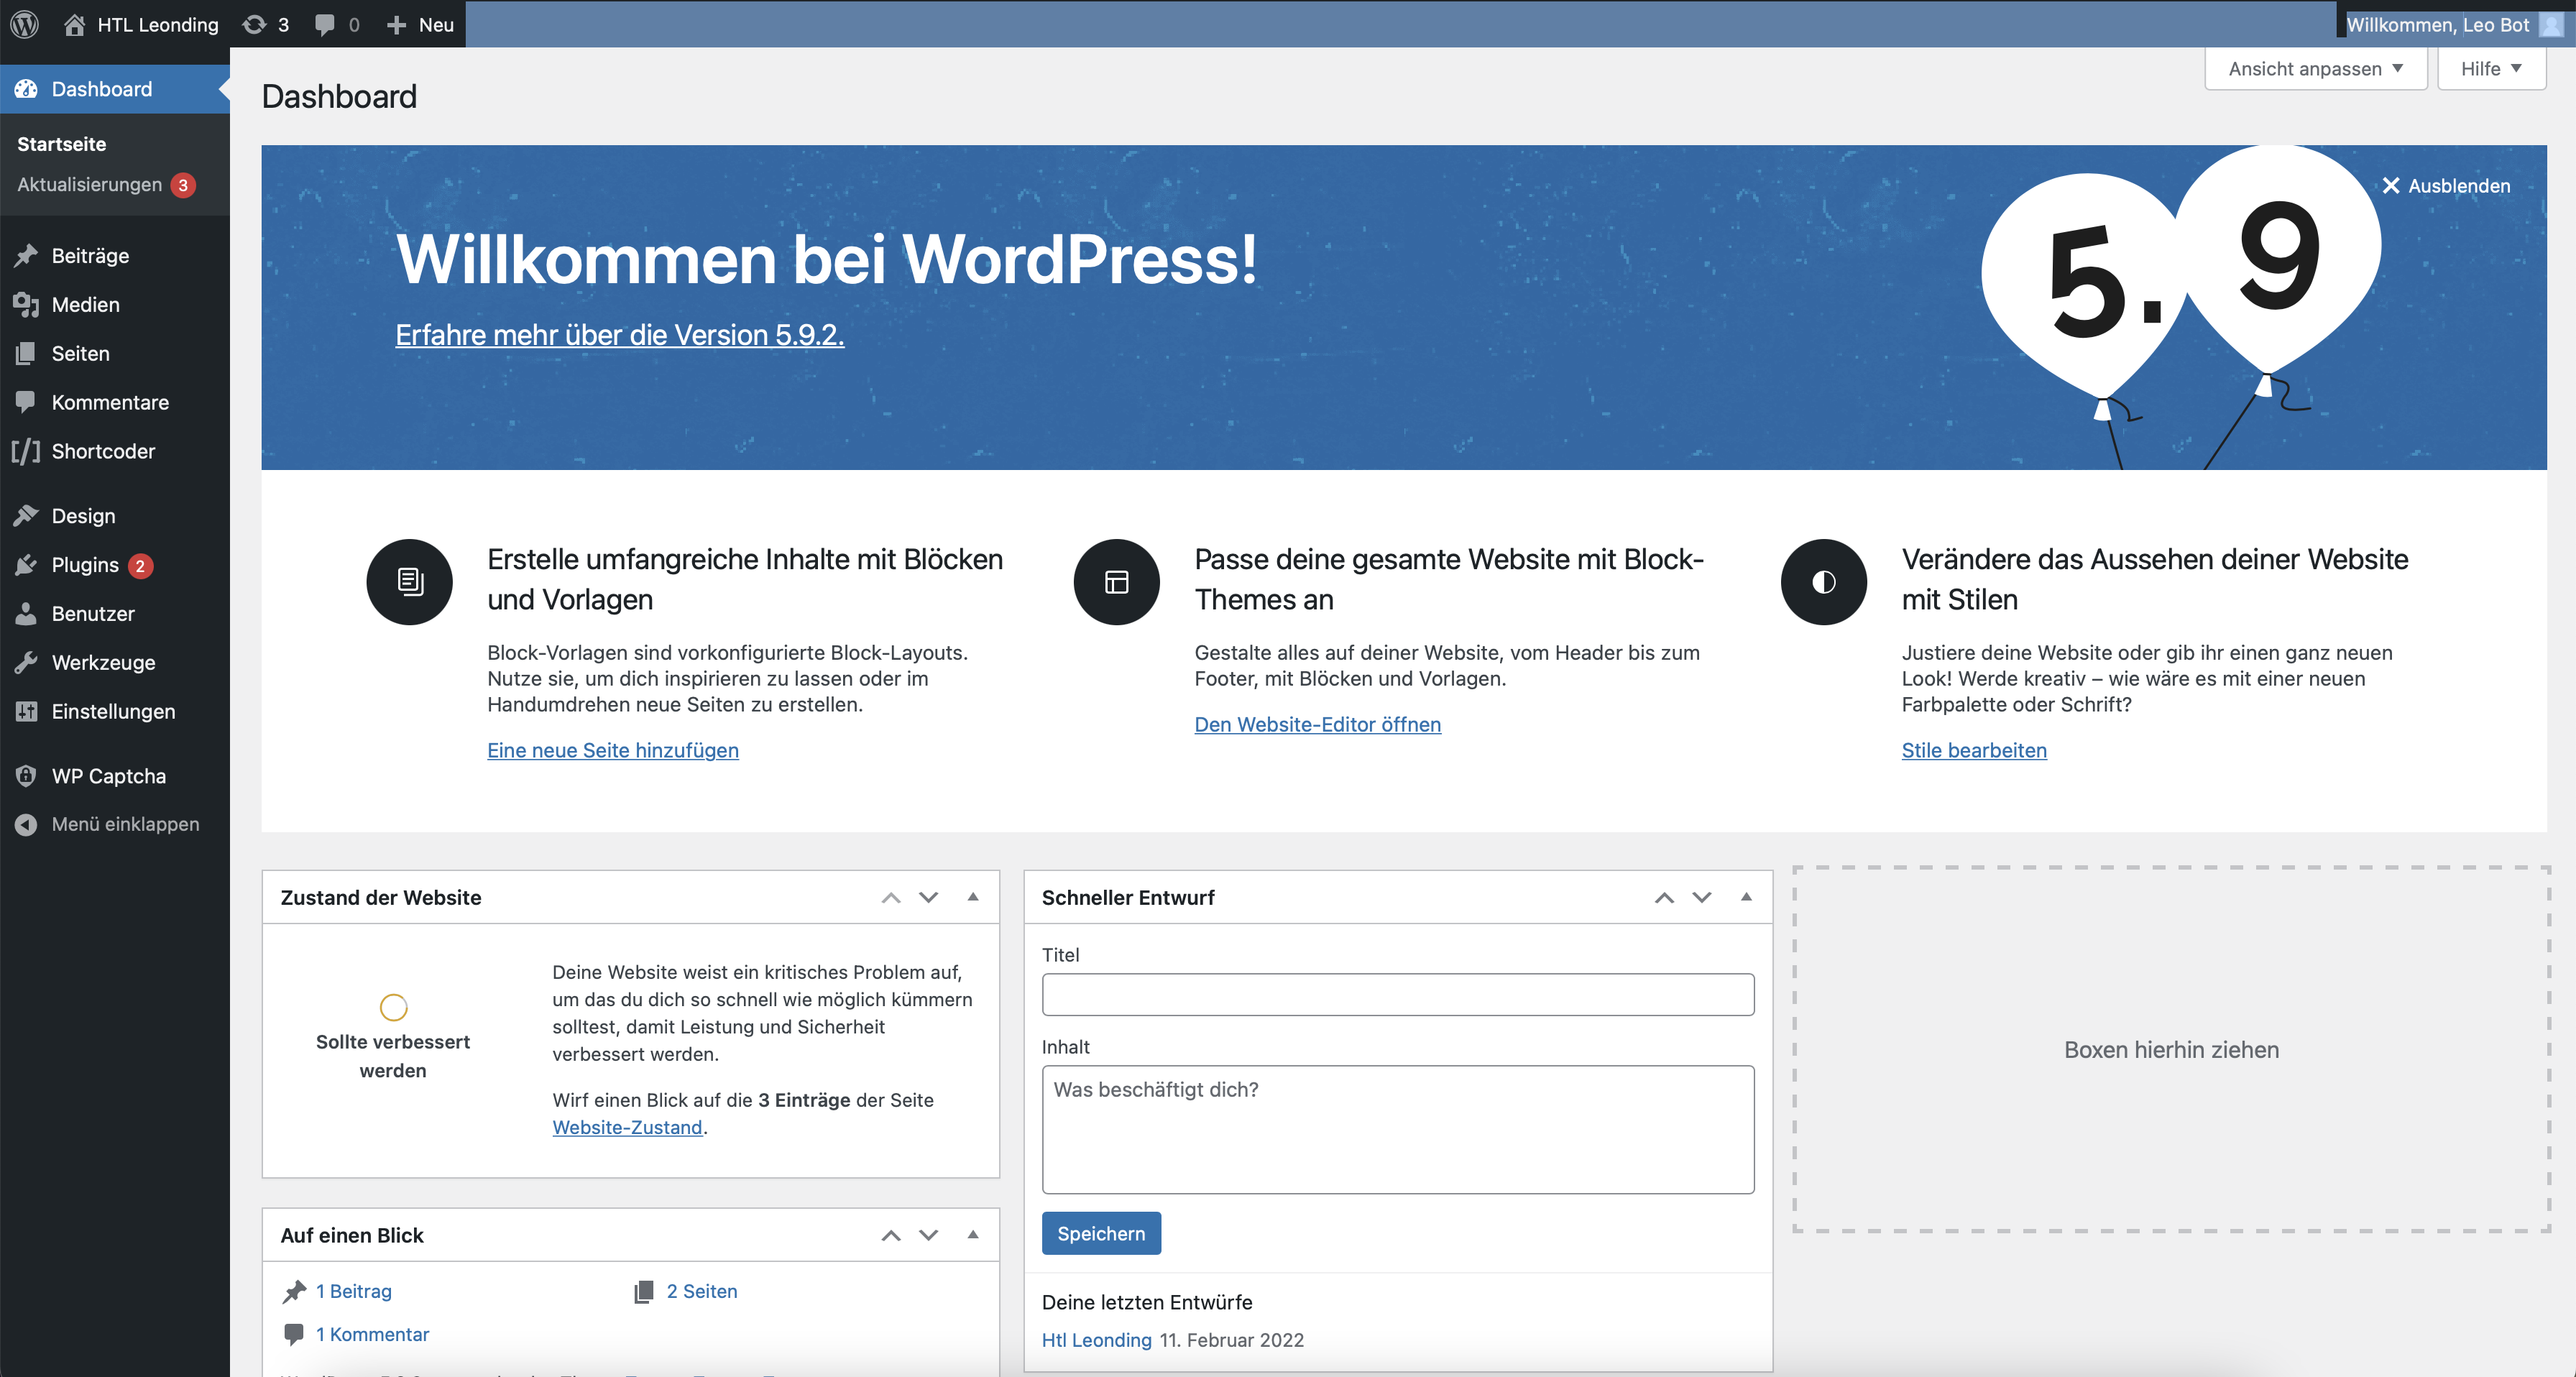
\includegraphics[scale=0.25]{pics/wordpresshome}
    \caption{Startseite WordPress}
    \label{fig:impl:wordpresshome}
\end{figure}


Auf WordPress können Beiträge verfasst werden, wie in Abbildung ~\ref{fig:impl:bloglist} zu erkennen ist.

\begin{figure}[hbt!]
    \centering
    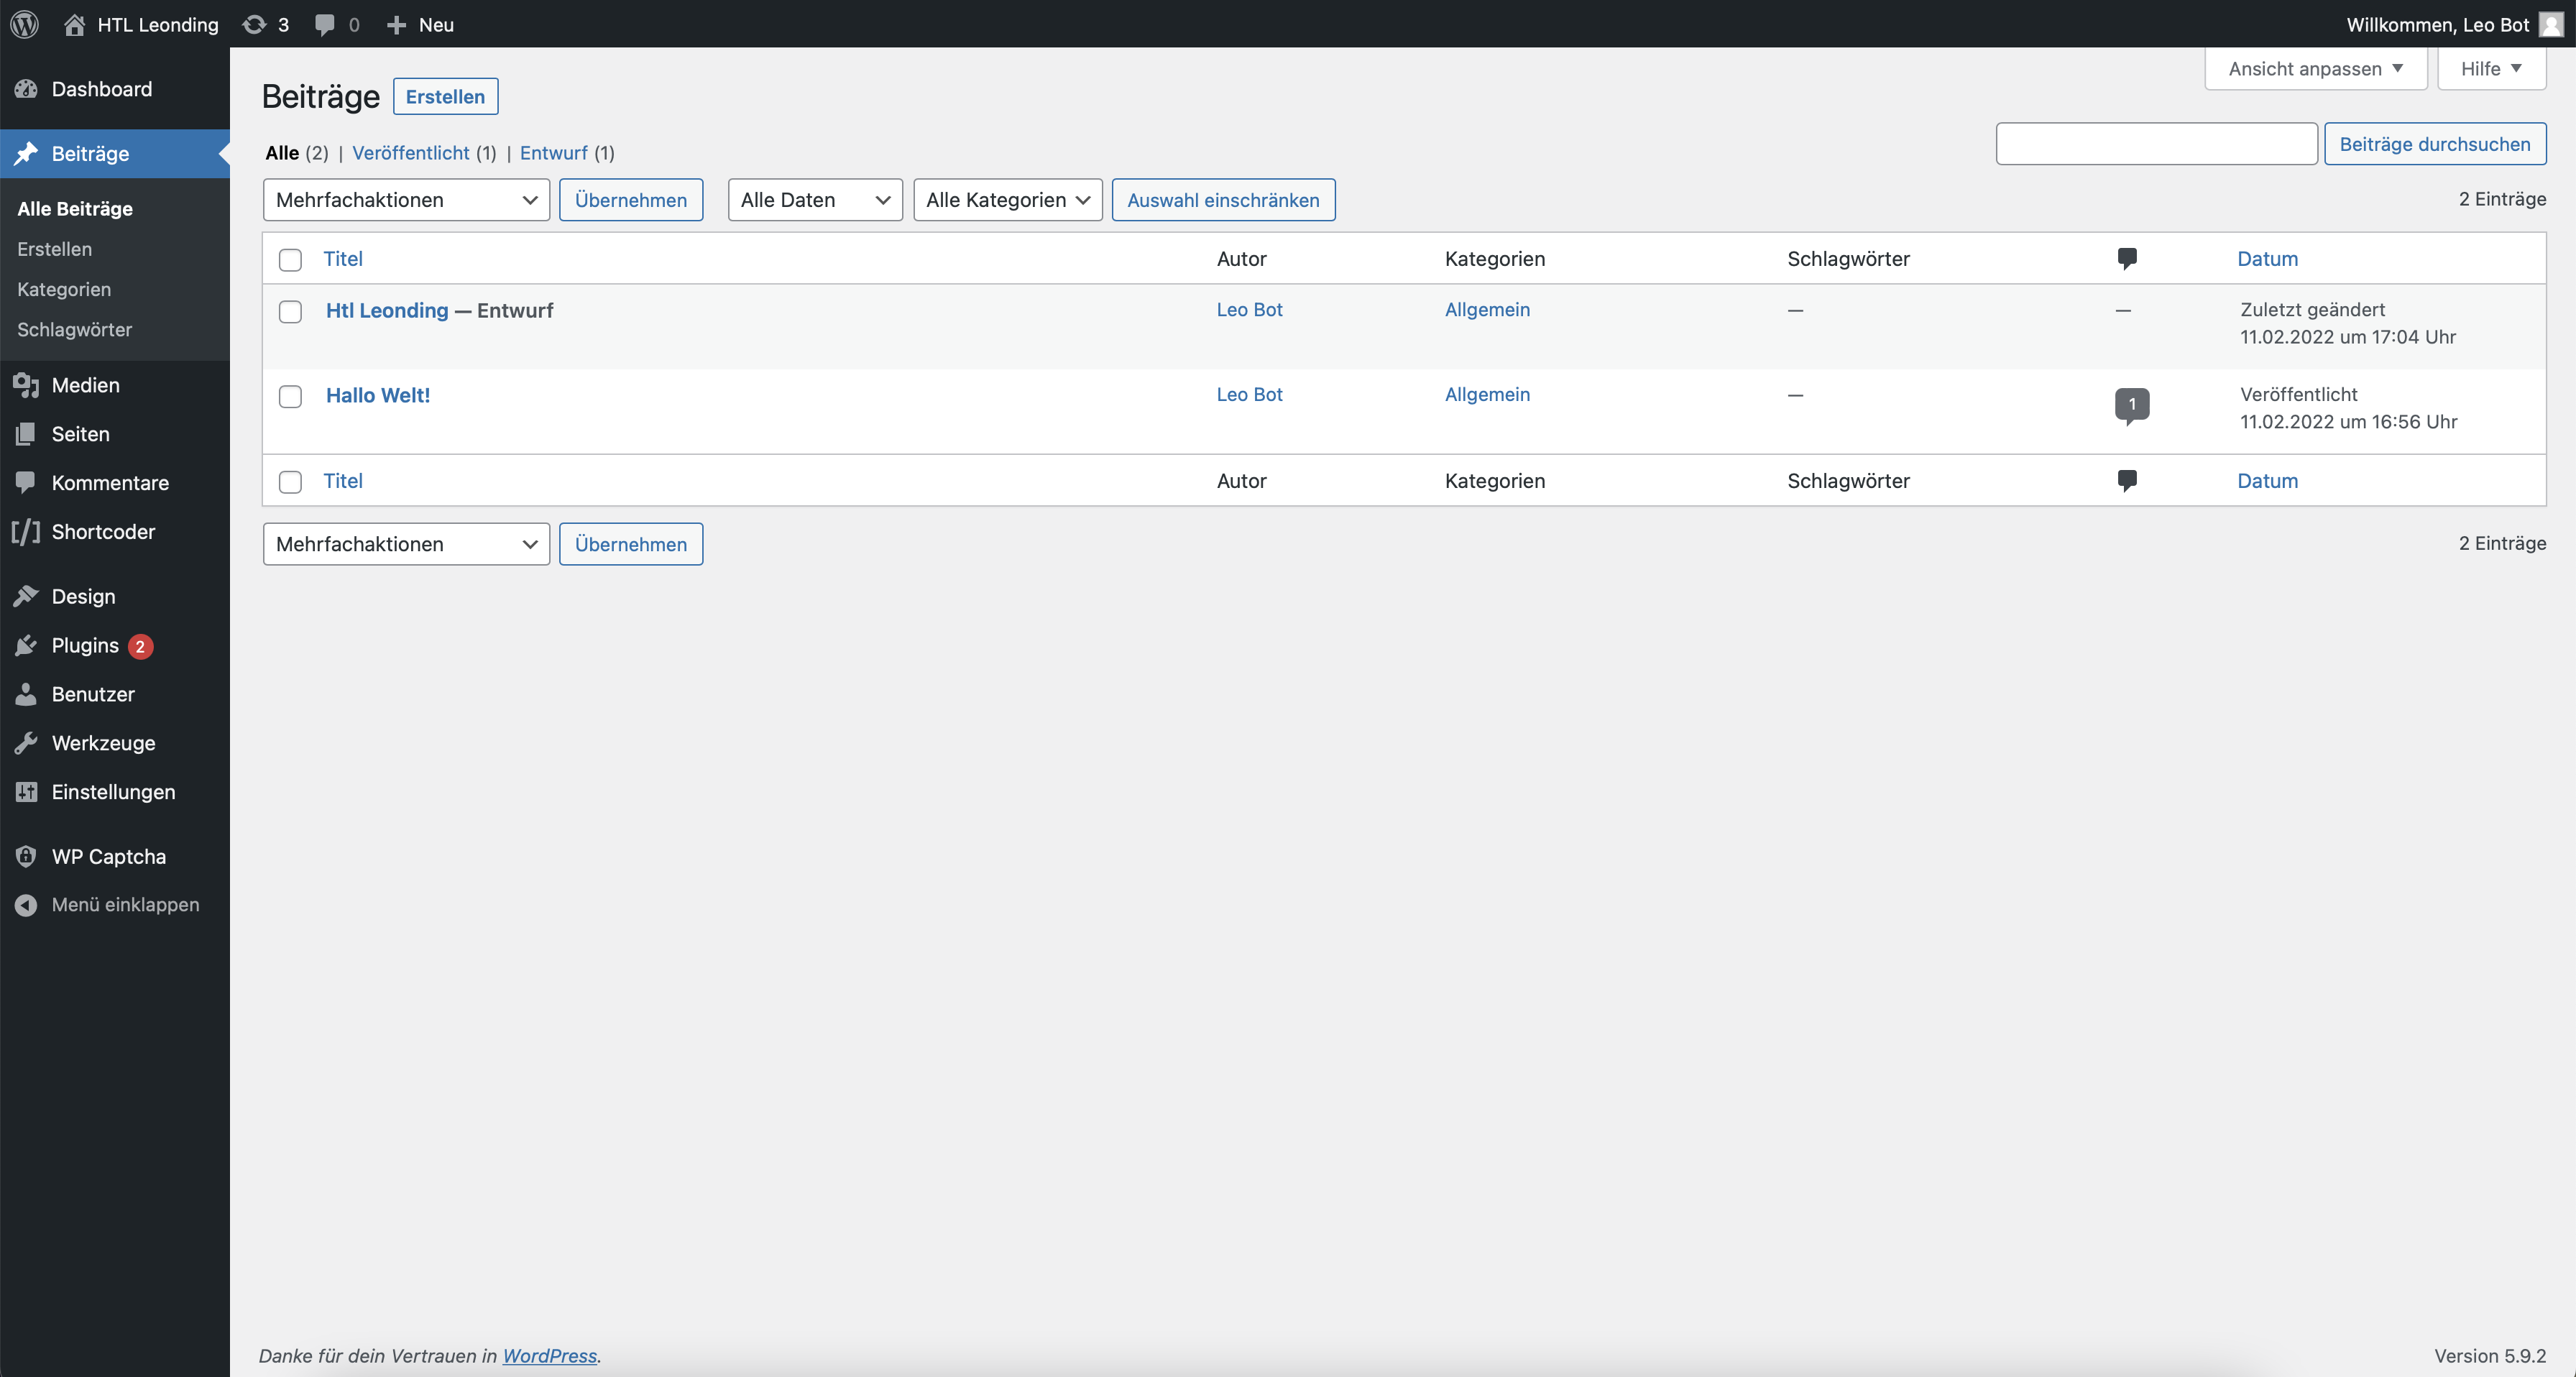
\includegraphics[scale=0.25]{pics/bloglist}
    \caption{WordPress Liste der Blogeinträge}
    \label{fig:impl:bloglist}
\end{figure}


Diese Beiträge können in einem eigenen Editor, der viele vorgefertigte Elemente bereits zur Verfügung stellt, verfasst werden.
Dies wird in Abbildung ~\ref{fig:impl:blogpost} beschrieben.

\begin{figure}[hbt!]
    \centering
    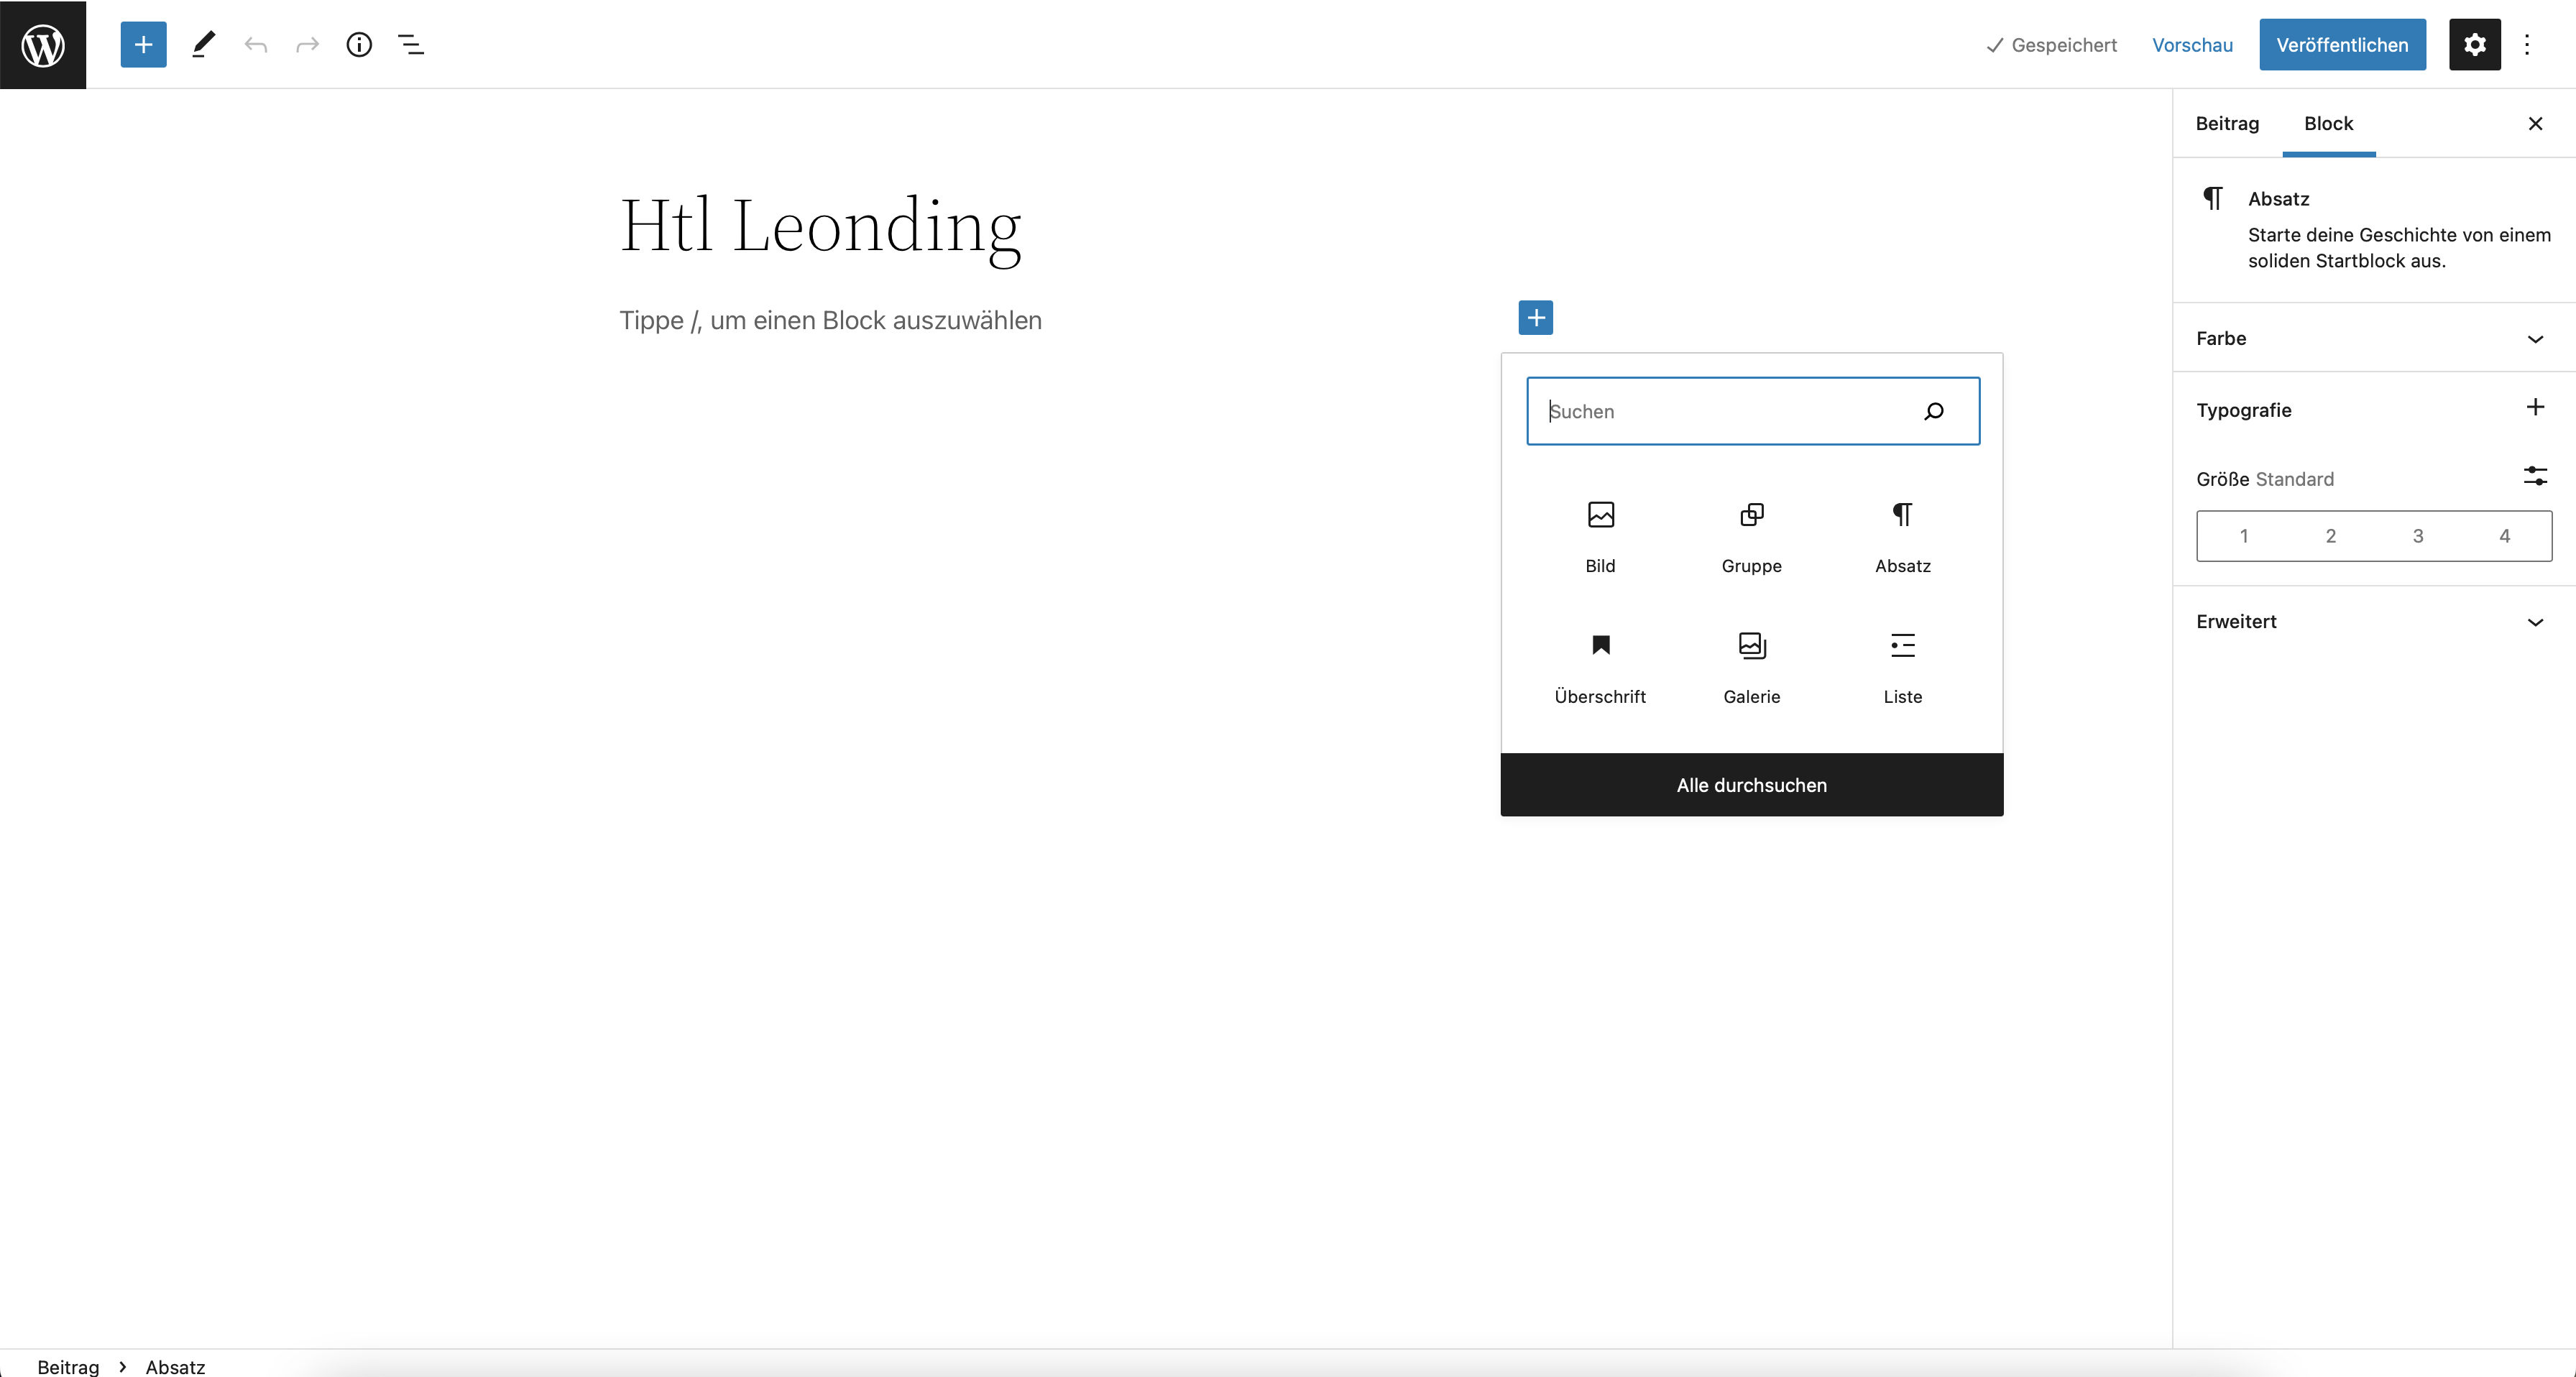
\includegraphics[scale=0.25]{pics/blogpost}
    \caption{Wordpress Blopost Editor}
    \label{fig:impl:blogpost}
\end{figure}
